
\section{note storiche}

\subsection{il numero $e$}

\begin{figure}
  \begin{center}
  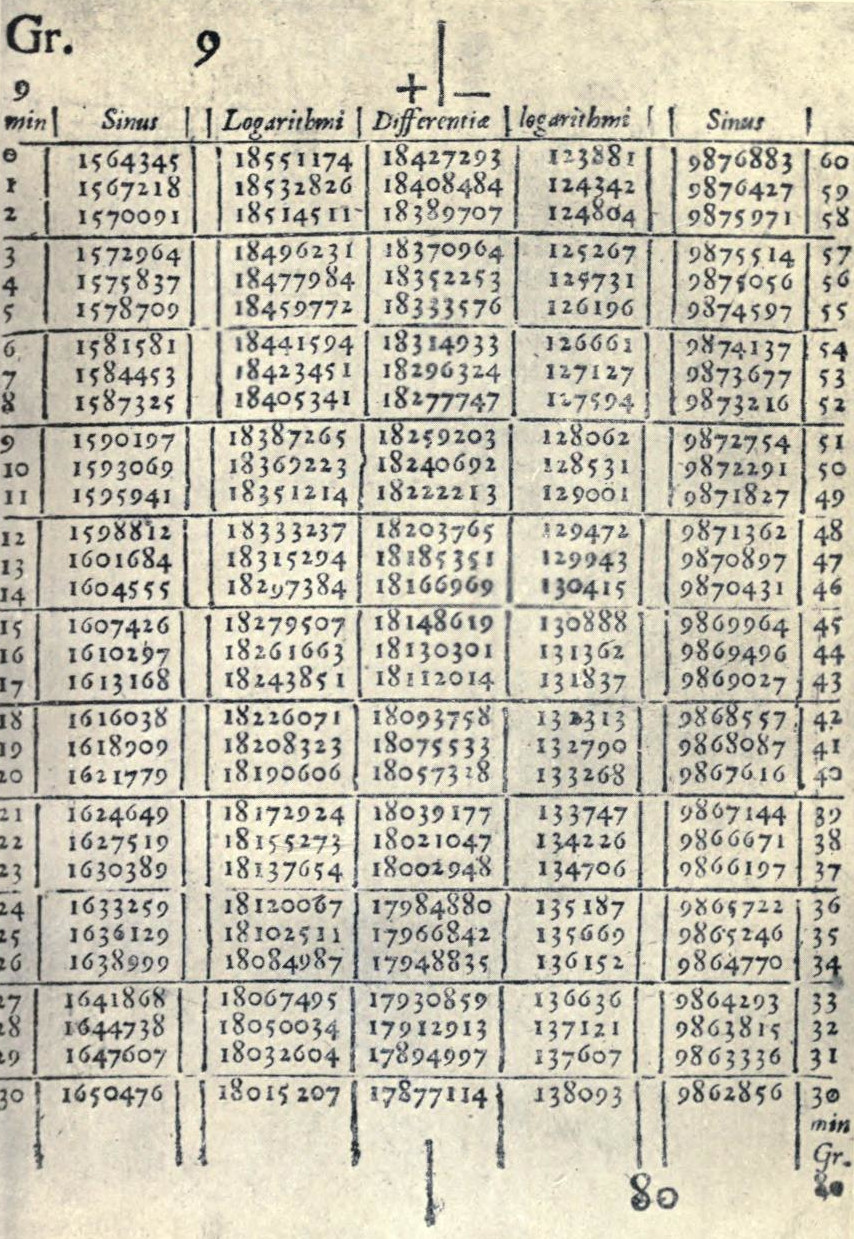
\includegraphics[width=10cm]{napier_tables.jpg}
  \end{center}
  \caption{Una pagina delle tavole calcolate da John Napier
  con i valori della funzione $\sin$ (Sinus) e del suo logaritmo
  (Logarithmi).
  In questa pagina ci sono i valori 
  per gli angoli dai 9 gradi (Gr.) ai 9 gradi e mezzo (i gradi 
  sessagesimali sono suddivisi in 60 minuti) e 
  dei loro complementari dagli 80 gradi e mezzo agli 81 gradi.
  Il codice scritto a pag.~\pageref{code:napier} permette
  di calcolare in pochi centesimi di secondo gli stessi valori
  mettendo anche in evidenza alcuni errori sulle ultime cifre decimali.
  Napier ci mise 20 anni a completare la stesura 
  delle tavole da 0 a 90 gradi.
  Se ad esempio volessimo calcolare il valore della tangente di $\alpha=9$ gradi 
  potremmo osservare che il logaritmo di $\tg \alpha$ 
  è la differenza tra il logaritmo di $\sin \alpha$ e il 
  logaritmo di $\cos \alpha$.
  Essendo il $\cos$ uguale al seno dell'angolo complementare 
  troviamo questo valore nella tabella in figura, 
  riga 0, colonna 
  \emph{Differenti\ae}: $1.8427293$ 
  (tutti i valori sono moltiplicati per $10^7$).
  Il valore cercato è l'esponenziale di questo 
  logaritmo e possiamo quindi calcolarlo cercando 
  lo stesso valore nella colonna \emph{Logarithmi}
  e prendendo il corrispondente valore nella colonna 
  \emph{Sinus}. Il valore è compreso tra i valori 
  della riga 6 e della riga 7. Più precisamente 
  differisce dal valore nella riga 7 
  $\frac{3842}{18143}$ volte quanto differisce il valore 
  della riga 6 dal valore della riga 7. 
  Applicando lo stesso rapporto ai valori trovati 
  nella colonna \emph{Sinus} si ottiene
  per interpolazione che al valore 
  della riga 7 (pari a 1.584453) và 
  sottratto 608 ottenendo quindi $\tg \alpha \approx 0.1583845$
  che differisce dal valore 
  esatto per meno di $10^{-7}$.
  }
  \label{fig:napier}
\end{figure}

\label{nota:Nepero}%
\index{Napier!John}%
\index{Nepero}%
\label{Euler!Leonhard}%
\label{Eulero}%
Nepero è l'italianizzazione del nome del
matematico scozzese \emph{John Napier} (1550-1617)
che per compilare le tavole della funzione seno
con una precisione di 7 cifre decimali ha introdotto 
per primo la funzione logaritmo (si veda la figura~\ref{fig:napier}).
E' interessante notare che Napier ha definito direttamente 
il logaritmo naturale senza introdurre il numero $e$ 
e senza fare alcun collegamento con la funzione esponenziale.
% https://archive.org/details/johnnapierinvent00hobsiala/page/18/mode/2up

\label{note:Bernoulli}%
\index{Bernoulli!Jacob}%
L'individuazione della costante $e$
è dovuta a \emph{Jacob Bernoulli} (1655--1705) nel 1683.
Bernoulli si chiedeva qual è l'interesse annuo effettivo
che si ottiene da un capitale che dia una rendita
giornaliera.
Se investo un capitale $c$ ad un tasso di interesse annuo 
pari a $r$, alla fine dell'anno mi viene restituito 
il capitale $c$ più un interesse $rc$.
Se divido il guadagno $rc$ per il numero di giorni che ci sono in 
un anno, posso considerare di aver avuto un guadagno giornaliero
pari a $\frac{r}{365} c$.
Se il guadagno giornaliero $\frac{r}{365} c$ mi venisse restituito 
immediatamente ogni giorno dell'anno, potrei reinvestire immediatamente 
il guadagno facendo aumentare il capitale durante l'anno.
In tal modo se parto con un capitale $c$ ogni giorno il mio capitale 
aumenterebbe di un fattore $1+\frac{r}{365}$ e
alla fine dell'anno avrei quindi un guadagno
pari a $\enclose{1+\frac{r}{365}}^{365} \approx e^r$ 
volte il capitale iniziale (interesse composto).

Il nome $e$ è stato introdotto da Eulero (Leonhard Euler 1707-1783).
%http://eulerarchive.maa.org//docs/originals/E853.pdf

\subsection{il teorema fondamentale dell'algebra}

La formula risolutiva per determinare le radici di un polinomio di secondo grado 
era già nota ai Babilonesi e sebbene i numeri complessi non erano noti 
(e neanche i numeri negativi) la stessa formula si applica 
nel caso generale e fornisce le radici complesse.

Lo studio delle equazioni di grado superiore al secondo si sviluppa invece 
nel 1500 ad opera dei matematici italiani Scipione del Ferro, 
Gerolamo Cardano, Niccolò Tartaglia e Lodovico Ferrari.
Essi determinano le formule risolutive per determinare le radici 
dei polinomi di terzo e quarto grado. 
Nell'applicare la formula risolutiva per l'equazione di terzo grado 
può capitare di dover calcolare la radice quadrata di un numero negativo
anche in situazioni in cui tutte le soluzioni alla fine risultano reali.
Ed è proprio in questo contesto che nascono i numeri complessi, come 
mero artificio matematico utilizzato per portare a termine il conto.

Successivamente Paolo Ruffini (1765-1822) e Niels Abel (1802-1829) dimostrarono che le equazioni 
di grado maggiore del quarto non ammettono una formula risolutiva 
esprimibile mediante radicali. 
Il criterio per determinare se un polinomio
ammette o meno formule risolutive è dovuto al matematico francese Évariste Galois
(1811-1832) che è considerato il fondatore della teoria dei gruppi.

Il teorema fondamentale dell'algebra, e cioè l'esistenza di radici 
complesse per polinomi di grado qualunque, viene dimostrato dal 
matematico tedesco Carl Friedrich Gauss (1777--1855). 
Questo teorema opera una svolta nel pensiero matematico in quanto 
per la prima volta si dà rilevanza ad un risultato astratto di esistenza 
slegato da una formula risolutiva. 
Il teorema non era affatto scontato, basti pensare che sia Leibniz 
che Nikolas Bernoulli erano convinti di aver trovato dei polinomi 
di quarto grado che non possono essere fattorizzati in contrasto 
con il teorema~\ref{th:fattorizzazione_polinomio_reale}.

\subsection{il problema isoperimetrico}

\label{note:isoperimetrico}%
\index{problema!isoperimetrico}%
Probabilmente già dal IX secolo a.C.\ era noto ai greci che 
la circonferenza, tra tutte le linee piane di lunghezza prefissata, 
è quella che racchiude la maggiore area (proprietà isoperimetrica).
Nell'Eneide Virgilio racconta che Didone si trovò ad affrontare 
un problema simile nella fondazione di Cartagine.
\index{Didone}%
\index{isoperimetrico!problema}%
\index{problema!isoperimetrico}%
\index{problema!di Didone}%
Salendo alla dimensione $n=3$ è naturale immaginare che 
la superficie che racchiude il volume maggiore con area fissata 
sia la sfera. 
Questo spiega il motivo per cui una goccia d'acqua, in assenza di gravità,
dovrebbe assumere una forma sferica: a causa della tensione superficiale, 
infatti, la superficie della goccia tenderà ad avere l'area minima.
Eulero (\emph{Leonhard Euler} 1707--1783)
\index{Euler!Leonhard}%
\index{Eulero}%
pensò di aver
trovato una dimostrazione
che si fondava su questo risultato:
presa una qualunque superficie chiusa nello spazio,
se questa non è una sfera è possibile
farne una piccola modifica in modo da ottenere una nuova superficie
che racchiude lo stesso volume ma che ha area strettamente inferiore.
Dirichlet (1805--1859) si accorse di un problema fondamentale 
nella dimostrazione di Eulero e nelle successive formalizzazioni di Steiner:
Eulero dimostrava che il minimo non può essere una superficie diversa dalla sfera,
ma non dimostrava che il minimo esiste.
Infatti Eulero dimostra che non ci può essere un minimo che non sia la sfera, 
ma non dimostra che il minimo esiste e quindi non è detto che la sfera sia il minimo: 
potrebbero esserci infinite superfici $S_1, S_2, \dots, S_n, \dots$ 
ognuna con area minore di quella della sfera e ognuna con area maggiore della successiva: 
$A(S_{n+1})< A(S_n)$. 
Per concludere il ragionamento di Eulero era necessario dimostrare 
che in una situazione del genere le superifici $S_n$ debbano, in qualche senso, 
tendere alla superficie sferica e che le loro aree debbano
tendere all'area della sfera. 
Karl Weiestrass (1815--1897)
\index{Weiestrass!Karl}%
si occupò di rifondare l'analisi in modo da rendere formali queste dimostrazioni.
La dimostrazione della proprietà isoperimetrica del cerchio e della sfera fu 
resa formale da Hermann Schwarz, 
\index{Schwarz!Hermann}%
uno studente della scuola di Weierstrass.
Il caso del cerchio viene usualmente attribuito a Steiner (1796--1863) in quanto 
sebbene non si fosse accorto, come Eulero, del problema dell'esistenza del minimo, 
aveva prodotto tutti gli strumenti necessari per completare la dimostrazione. 

La formulazione del problema isoperimetrico nella sua massima generalità 
(cioè per insiemi anche non regolari, e in dimensione qualunque)
è dovuta al matematico italiano Ennio De Giorgi (1928--1996)
\index{De Giorgi!Ennio}%
che formalizzò il concetto di perimetro introdotto
da Renato Caccioppoli (1904--1959).%
\index{Caccioppoli!Renato}%
\index{Caccioppoli!perimetro}%
